\chapter{Instalación de idioma español en WordPress}
En primera instancia, el idioma del WordPress puede no ser muy relevante. El idioma por defecto (inglés) es más universal que otros  como el español, y la  documentación, preguntas frecuentes, tutoriales y resolución de problemas generalmente se encuentra más fácilmente si se busca en inglés. Sin embargo, a la hora de prestar soporte y documentación para los usuarios del clúster, la gran mayoría son nacidos en Costa Rica, y por más extendido que esté el inglés, no se puede asumir que los usuarios dominan el idioma. Debido a esto, para facilitar el soporte para los usuarios, se opta por instalar el idioma español en el WordPress.

Lo primero que se debe hacer es descargar WordPress en el idioma deseado, en este caso Castellano (es\_ES) y se extrae los contenidos del archivo. Dentro viene los plugins de idioma, los cuales simplemente se deben copiar a la carpeta donde se encuentra la instalación activa de WordPress, y reiniciar el servicio. Debemos asegurarnos de  que la versión en español de WordPress a descargar sea la misma que la versión instalada (versión 4.3.1 al momento de redactar este documento). A continuación se detallan los pasos a seguir \cite{wplang}:
%%%%%%%%%%%%%%%%%%%%%%%%%%%%%%%%%%%%%%%%%%%%%%%%%%%%%%%%%%%%%%%%%%%%%
\lstinputlisting{wp_spanish.sh}
%%%%%%%%%%%%%%%%%%%%%%%%%%%%%%%%%%%%%%%%%%%%%%%%%%%%%%%%%%%%%%%%%%%%%
Una vez hecho esto, nos dirigimos a la página administrativa de WordPress \url{http://cluster.cenat.ac.cr/wordpress/wp-admin/} e iniciamos sesión. Nos dirigimos a Settings/Ajustes y a configuración general. De ahí bajamos hasta que veamos la opción Site Language, donde procedemos a cambiar el idioma al recién instalado Español,  tal y como se muestra en la figura \ref{fig:lang:01}.
%%%%%%%%%%%%%%%%%%%%%%%%%%%%%%%%%%%%%%%%%%%%%%%%%%%%%%%%%%%%%%%%%%%%%
\begin{figure}[H]
\centering
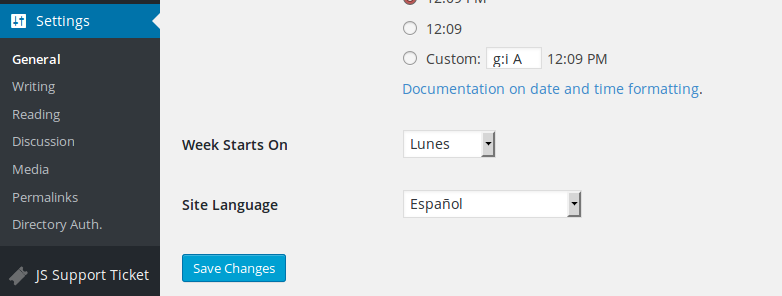
\includegraphics[width=0.5\textwidth]{lang_settings00.png}
\caption{Cambio de idioma del WordPress.}
\label{fig:lang:01}
\end{figure}
%%%%%%%%%%%%%%%%%%%%%%%%%%%%%%%%%%%%%%%%%%%%%%%%%%%%%%%%%%%%%%%%%%%%%
Si todo ha  transcurrido sin problemas, el sitio en general debería verse como en la figura \ref{fig:lang:02}. Esto concluye la guía de cómo instalar el idioma español. El proceso puede replicarse  para  instalar otros idiomas si fuese necesario, haciendo los cambios mínimos necesarios.
%%%%%%%%%%%%%%%%%%%%%%%%%%%%%%%%%%%%%%%%%%%%%%%%%%%%%%%%%%%%%%%%%%%%%
\begin{figure}[H]
\centering
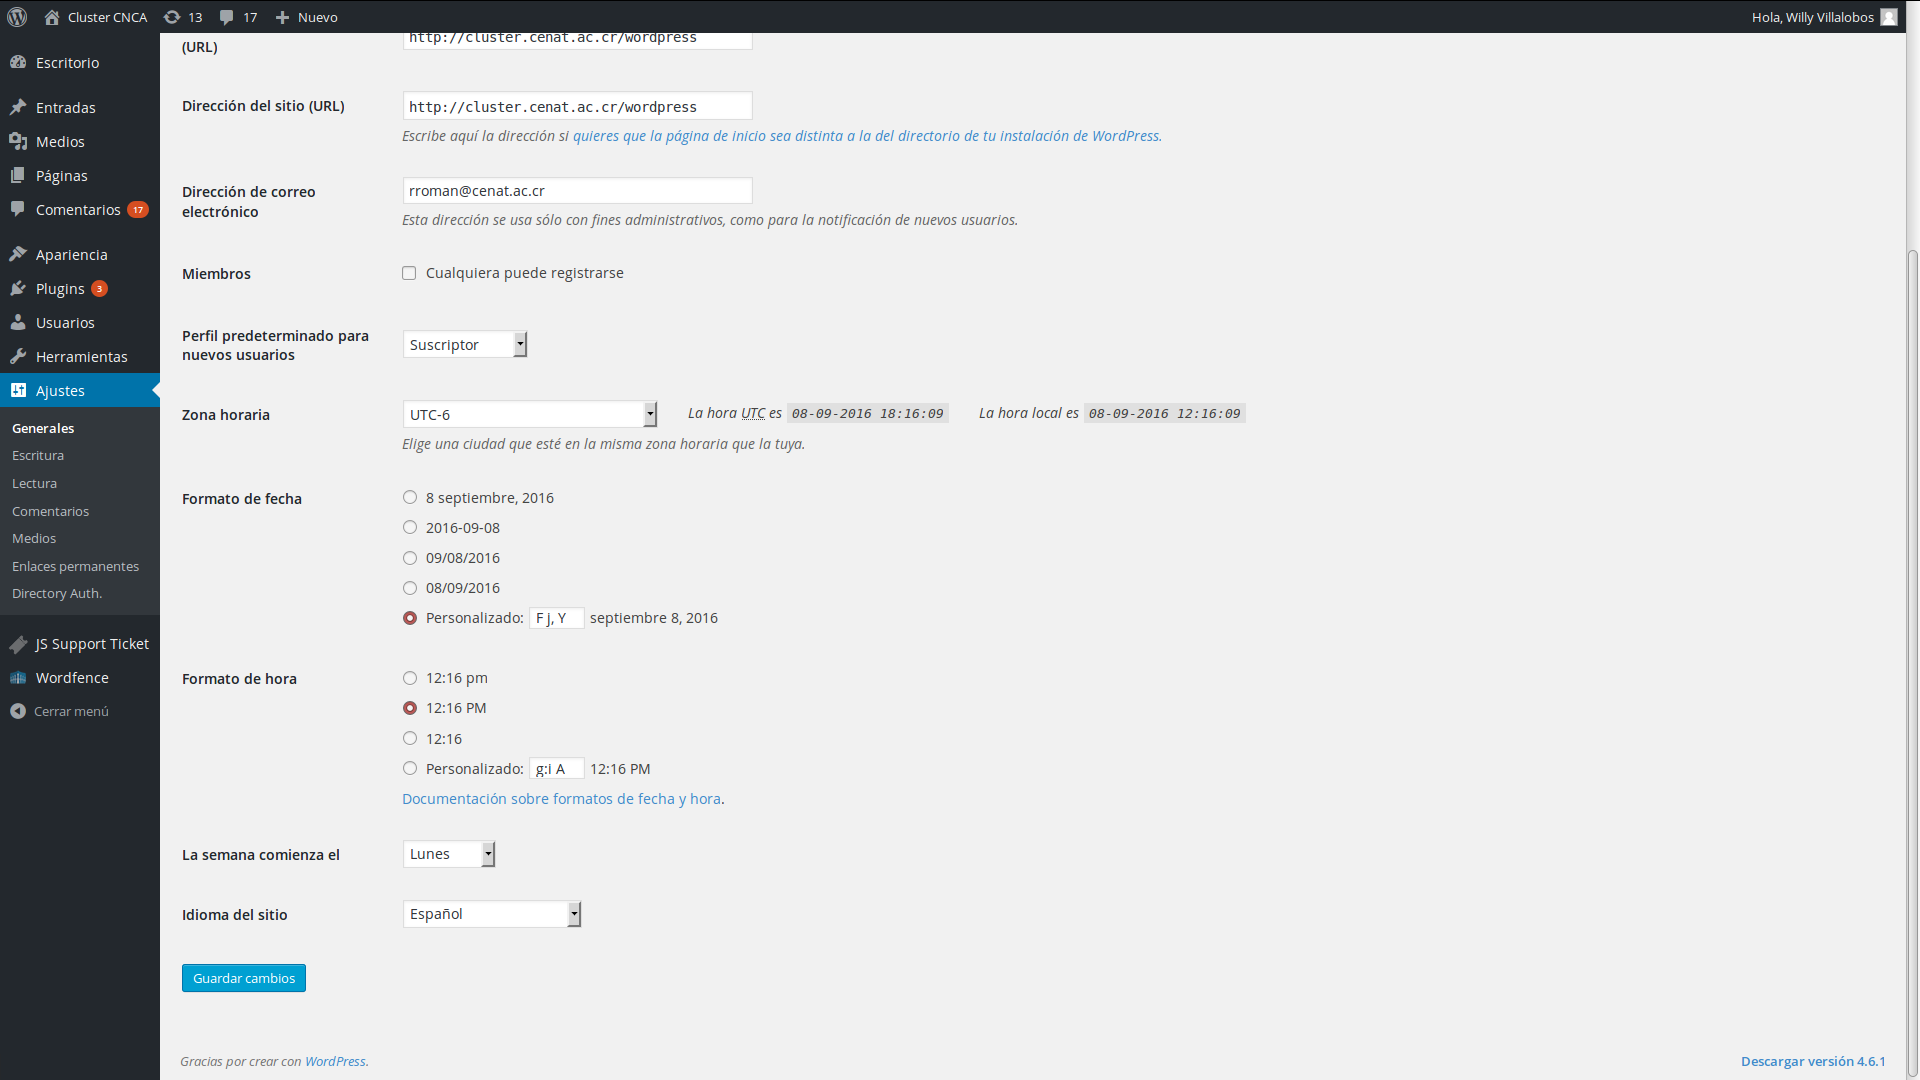
\includegraphics[width=0.7\textwidth]{lang_settings01.png}
\caption{Sitio administrativo del WordPress en idioma español.}
\label{fig:lang:02}
\end{figure}
%%%%%%%%%%%%%%%%%%%%%%%%%%%%%%%%%%%%%%%%%%%%%%%%%%%%%%%%%%%%%%%%%%%%%
\clearpage